% !TEX program = xelatex
% 공통수학2 · Ⅲ. 함수와 그래프 · 2. 유리함수와 무리함수 · 01 유리함수 · 2/2차시
\documentclass[11pt,a4paper]{article}
\usepackage{kotex}
\usepackage{iftex}
\ifPDFTeX\else
  \setmainhangulfont{Noto Serif CJK KR}
  \setsanshangulfont{Noto Sans CJK KR}
\fi
\usepackage[margin=2.1cm]{geometry}
\usepackage{parskip}
\usepackage{enumitem}
\usepackage{array}
\usepackage{tabularx}
\usepackage{booktabs}
\usepackage{xcolor}
\usepackage{amssymb}
\usepackage{tikz}
\usepackage[most]{tcolorbox}
\usepackage{fancyhdr}
\usepackage{titlesec}

\definecolor{goldc}{HTML}{B07C22}
\definecolor{goldstrong}{HTML}{8A5F16}
\definecolor{indigoc}{HTML}{2B3B57}
\definecolor{indigosoft}{HTML}{6E82A6}
\definecolor{linec}{HTML}{D6DACB}
\definecolor{surface2}{HTML}{E4E8DC}
\definecolor{notebg}{HTML}{FBF3E3}
\definecolor{inksoft}{HTML}{52604F}

\titleformat{\section}{\normalfont\sffamily\bfseries\large\color{indigoc}}{\thesection}{0.6em}{}
\titlespacing{\section}{0pt}{16pt}{8pt}
\newtcolorbox{ideabox}{enhanced, breakable, colback=white, colframe=goldc, boxrule=0.5pt, leftrule=3pt, arc=2pt, left=10pt, right=10pt, top=8pt, bottom=8pt}
\newtcolorbox{calloutbox}{enhanced, breakable, colback=white, colframe=indigosoft, boxrule=0.5pt, leftrule=3pt, arc=2pt, left=10pt, right=10pt, top=7pt, bottom=7pt}
\newtcolorbox{notebox}{enhanced, breakable, colback=notebg, colframe=goldc, boxrule=0.5pt, leftrule=3pt, arc=2pt, left=10pt, right=10pt, top=7pt, bottom=7pt}
\newtcolorbox{answerbox}{enhanced, breakable, colback=white, colframe=linec, boxrule=0.5pt, arc=2pt, left=10pt, right=10pt, top=7pt, bottom=7pt}
\newcommand{\lessonbanner}[3]{%
  \begin{tcolorbox}[enhanced, colback=indigoc, colframe=indigoc, boxrule=0pt, arc=0pt,
    left=14pt, right=14pt, top=14pt, bottom=10pt, borderline south={2.4pt}{0pt}{goldc}, fontupper=\color{white}]
    {\sffamily\footnotesize\color{white!85!black} #1}\\[4pt]{\sffamily\bfseries\Large #2}\\[3pt]{\sffamily\small\color{white!88!black} #3}
  \end{tcolorbox}}
\pagestyle{fancy}\fancyhf{}\renewcommand{\headrulewidth}{0pt}
\fancyfoot[L]{\footnotesize\color{inksoft} 공통수학2 · 2026학년도 2학기 · 지평선고등학교}
\fancyfoot[R]{\footnotesize\color{inksoft} 교사용 지도안 -- 배포 금지}

\begin{document}
\lessonbanner{공통수학2 · Ⅲ. 함수와 그래프 · 2. 유리함수와 무리함수}{01 유리함수 --- 2/2차시}{유리함수의 그래프 · 교사용 지도안 (2026학년도 2학기)}
\vspace{10pt}

\noindent\begin{tabularx}{\linewidth}{@{}>{\bfseries\color{indigoc}}p{2.6cm}X@{}}
\toprule
대상 & 고1 · 2개 반 · 반당 13명 \\
차시 & 50분 (도입 10 · 전개 30 · 정리 10) \\
성취기준 & 유리함수 $y=\dfrac{k}{x-p}+q$의 그래프를 그리고, 점근선을 구할 수 있다. \\
선행 학습 & 39차시 --- 유리함수의 뜻과 정의역, 14차시 --- 평행이동 \\
\bottomrule
\end{tabularx}

\section{학습 목표 \& Big Idea}
\begin{ideabox}
\textbf{\color{goldstrong}영속적 이해 (Big Idea)}\\
모든 유리함수 $y=\dfrac{k}{x-p}+q$의 그래프는 가장 단순한 $y=\dfrac{k}{x}$의 그래프를 평행이동한 것이다. 점근선은 그래프가 다가가지만 결코 닿지 않는 경계이며, 그 위치가 곧 평행이동한 만큼을 보여 준다.
\vspace{4pt}
\small\color{inksoft} 핵심개념: \textbf{점근선} \quad\textbullet\quad 핵심개념: \textbf{평행이동} \quad\textbullet\quad 일반화: \textbf{모든 유리함수의 그래프는 하나의 원형에서 평행이동으로 만들어진다}
\end{ideabox}
\begin{calloutbox}
\textbf{차시 학습 목표}
\begin{itemize}[leftmargin=1.4em, itemsep=2pt, topsep=4pt]
  \item $y=\dfrac{k}{x}$의 그래프의 성질(원점 대칭, 점근선 $x=0$, $y=0$)을 설명할 수 있다.
  \item $y=\dfrac{k}{x-p}+q$의 그래프를 그리고, 정의역·치역·점근선을 구할 수 있다.
\end{itemize}
\end{calloutbox}

\section{질문의 연결}
\begin{tabularx}{\linewidth}{@{}>{\bfseries\color{indigoc}\small}p{2.4cm}X@{}}
사실적 질문 & $y=\dfrac{k}{x-p}+q$의 그래프의 점근선은 각각 무엇일까? \\[6pt]
개념적 질문 & 그래프가 점근선에 무한히 가까워지지만 결코 닿지 않는 이유는 무엇일까? \\[6pt]
논쟁적 질문 & 목표에 계속 가까워지지만 완전히 도달하지는 못하는 상황을 우리 삶에서 찾을 수 있을까? 그것은 `실패'일까, 아니면 다른 의미가 있을까? \\
\end{tabularx}

\section{수업 흐름}
\begin{tabularx}{\linewidth}{@{}>{\centering\arraybackslash}p{1.6cm}X>{\raggedright\arraybackslash\small}p{3.1cm}@{}}
\toprule
\textbf{단계} & \textbf{활동 \& 발문} & \textbf{ATL / VTR} \\
\midrule
\textcolor{goldstrong}{\textbf{도입}}\newline\footnotesize 10분 &
\textbf{마음공부 (2분)} --- 유무념 대조.\newline
\textbf{생각 열기 (8분)} --- $y=\dfrac1x$에서 $x=0.1,0.01,0.001,\ldots$일 때 $y$값을 표로 만들며 $x$가 $0$에 가까워질수록 $y$가 한없이 커짐을 확인. &
ATL: 사고(극한적 직관)\newline VTR: See-Think-Wonder \\
\addlinespace
\textcolor{goldstrong}{\textbf{전개}}\newline\footnotesize 30분 &
\textbf{$y=\dfrac kx$의 그래프 (12분)} --- 원점에 대하여 대칭, 점근선 $x=0$, $y=0$, $k>0$이면 제1·3사분면, $k<0$이면 제2·4사분면에 위치함을 그래프로 확인 $\to$ 문제 1.\newline
\textbf{평행이동 (10분)} --- $y=\dfrac{k}{x-p}+q$는 $y=\dfrac kx$를 $x$축 방향 $p$, $y$축 방향 $q$만큼 평행이동한 것 --- 점근선도 $x=p$, $y=q$로 함께 이동 $\to$ 예제, 문제 2.\newline
\textbf{종합 문제 (8분)} --- 지난 시간 변형한 식을 그래프로 완성 $\to$ 문제 3, 문제 4(그래프 정보로 식 역산). &
ATT: 촉진자 역할\newline ATL: 기하적 추론·대수적 조작 \\
\addlinespace
\textcolor{goldstrong}{\textbf{정리}}\newline\footnotesize 10분 &
\textbf{개념 연결 질문 (5분)} --- ``$y=\dfrac{k}{x-p}+q$의 그래프를 한눈에 그리려면 무엇부터 표시해야 할까?''\newline
\textbf{성찰 (5분)} --- 감사 일기 1문장 + 다음 차시 예고(무리함수). &
마음공부 · 감사 일기 \\
\bottomrule
\end{tabularx}

\begin{calloutbox}
\textbf{지도상의 유의점} --- 점근선을 먼저 그리고 그 교점(점근선의 교점, 대칭의 중심)을 표시한 뒤 그래프를 그리는 순서를 강조한다. 점근선은 그래프에 포함되지 않는 `가상의 선'이며 점선으로 표시함을 짚어 준다.
\end{calloutbox}

\section{형성평가 \& 답안}
\begin{minipage}[t]{0.48\linewidth}
\begin{answerbox}
\textbf{문제 1} \quad $y=\dfrac2x$의 그래프의 점근선, 정의역, 치역을 구하시오.

\vspace{4pt}
\centering
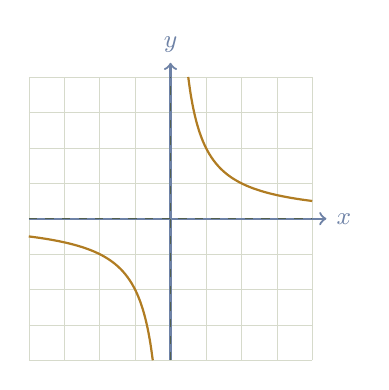
\begin{tikzpicture}[scale=0.45]
  \draw[step=1cm, linec, very thin] (-4,-4) grid (4,4);
  \draw[->, thick, indigosoft] (-4,0) -- (4.4,0) node[right,font=\small]{$x$};
  \draw[->, thick, indigosoft] (0,-4) -- (0,4.4) node[above,font=\small]{$y$};
  \draw[dashed, inksoft] (-4,0) -- (4,0);
  \draw[dashed, inksoft] (0,-4) -- (0,4);
  \draw[thick, goldc, domain=0.5:4, samples=60, smooth] plot(\x,{2/\x});
  \draw[thick, goldc, domain=-4:-0.5, samples=60, smooth] plot(\x,{2/\x});
\end{tikzpicture}

\vspace{4pt}
\raggedright\textbf{\color{goldstrong}답} \; 점근선: $x=0$, $y=0$. 정의역 $\{x\mid x\neq0\}$, 치역 $\{y\mid y\neq0\}$. $k=2>0$이므로 제1·3사분면에 위치.
\end{answerbox}
\end{minipage}\hfill
\begin{minipage}[t]{0.48\linewidth}
\begin{answerbox}
\textbf{문제 2} \quad $y=\dfrac{3}{x-1}+2$의 그래프를 그리고, 점근선·정의역·치역을 구하시오.

\vspace{4pt}
\centering
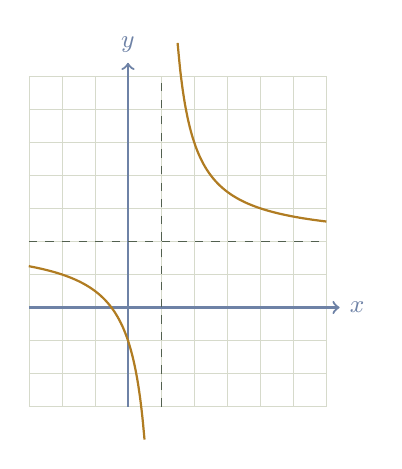
\begin{tikzpicture}[scale=0.42]
  \draw[step=1cm, linec, very thin] (-3,-3) grid (6,7);
  \draw[->, thick, indigosoft] (-3,0) -- (6.4,0) node[right,font=\small]{$x$};
  \draw[->, thick, indigosoft] (0,-3) -- (0,7.4) node[above,font=\small]{$y$};
  \draw[dashed, inksoft] (1,-3) -- (1,7);
  \draw[dashed, inksoft] (-3,2) -- (6,2);
  \draw[thick, goldc, domain=1.5:6, samples=60, smooth] plot(\x,{3/(\x-1)+2});
  \draw[thick, goldc, domain=-3:0.5, samples=60, smooth] plot(\x,{3/(\x-1)+2});
\end{tikzpicture}

\vspace{4pt}
\raggedright\textbf{\color{goldstrong}답} \; 점근선: $x=1$, $y=2$. 정의역 $\{x\mid x\neq1\}$, 치역 $\{y\mid y\neq2\}$.
\end{answerbox}
\end{minipage}

\vspace{6pt}
\begin{answerbox}
\textbf{문제 3} \quad 지난 시간에 변형한 $y=\dfrac{2x+1}{x-1}=\dfrac{3}{x-1}+2$의 그래프의 점근선을 구하시오.\\[4pt]
\textbf{\color{goldstrong}답} \; 점근선 $x=1$, $y=2$ (문제 2와 동일한 그래프임을 확인).
\end{answerbox}
\begin{answerbox}
\textbf{문제 4} \quad 점근선이 $x=-3$, $y=1$이고 점 $(-2,3)$을 지나는 유리함수의 식을 구하시오.\\[4pt]
\textbf{\color{goldstrong}답} \; $y=\dfrac{k}{x+3}+1$로 놓고 $(-2,3)$ 대입: $3=\dfrac{k}{1}+1 \Rightarrow k=2$. \; $y=\dfrac{2}{x+3}+1$
\end{answerbox}

\section{성취수준 (이 차시 범위)}
\begin{tabularx}{\linewidth}{@{}>{\bfseries\color{goldstrong}}p{0.9cm}X@{}}
\toprule
A & 점근선과 평행이동의 관계를 논리적으로 설명하고, 그래프 정보로부터 유리함수의 식을 역으로 구할 수 있다. \\
B & $y=\dfrac{k}{x-p}+q$의 그래프를 그리고, 점근선·정의역·치역을 구할 수 있다. \\
C & 안내에 따라 $y=\dfrac kx$의 그래프를 그리고 점근선을 구할 수 있다. \\
D & 유리함수의 점근선이 무엇인지 안다. \\
E & $y=\dfrac kx$ 꼴의 함수를 안다. \\
\bottomrule
\end{tabularx}

\section{다음 차시}
\begin{calloutbox}
\textbf{02 무리함수 --- 1/1차시.} 근호를 포함한 무리함수의 뜻, 정의역, 그래프를 다룬다.
\end{calloutbox}
\end{document}
